\section{SSQ Ranking}
\label{sec:ssq}
In order to match a new query with a SSQ within our data store, we
have defined similarity measures between the ontologies of the new
query and the candidate SSQs. These measures capture the distance
between the ontology classes, properties, and individuals at the
conceptual level in addition to simply matching URIs. The similarity
measures are implemented in two scenarios: \textit{on-line execution}
and \textit{off-line mode}. The \textit{on-line execution} is time
sensitive and is used primarily for relating newly defined SSQs to the
SSQs in the store. During \textit{off-line execution}, the system
clusters similar SSQs.

The similarity measure for the SSQ ontologies is determined by the
following components.
\begin{enumerate}
    \item QueryClass: an OWL class and the root of the SSQ ontology
      structure.
    \item hasRealm: an OWL object property with its domain as the SSQ
      Query class and its range as a realm class.
    \item Contexts such as who, what, when, and where are OWL object
      properties, whose domains are the query classes and ranges are
      OWL classes.
    \item SSQClass: an OWL class which is created from the components
      described above.
\end{enumerate}
Based on this ontology structure and the execution scenarios, we have
created an algorithm for finding the matches between SSQ
ontologies. It is based on class divergence, which is motivated by the
concept of multiple dispatch in CLOS \cite{95411} and Dylan
programming \cite{DBLP:conf/oopsla/BarrettCHMPW96} for generic
function type matches. We consider the realm class and context
property ranges for determining SSQ similarity. Once we have the similarity measures between the user defined SSQ and relevant QRMs in the store, we can order the relevant QRMs. The order provides a ranking for the results to the user. Subsections \ref{sec:ctd}, and \ref{sec:oqom} describe about this in detail.


\subsection{Class Divergence}
\label{sec:ctd}
We employ a measure of compatibility, which we call \textit{class
  divergence}, between a source class and a target class using the
\textit{topological structure} of the context classes in the
ontology. We write $S \prec T$ for the reflexive transitive closure of
the superclass relation. Let $d(P,Q)$ represent the hop distance in
the directed ontology inheritance graph from $P$ to $Q$. The
divergence between a source and target class ranges from zero (for
identical classes) to one (for incompatible classes).  Let $S$ be the
source class, $T$ be the target class, and let $C$ be a common
ancestor class of $S$ and $T$ minimizing $d(S,C) + d(T,C)$. The class
divergence between $S$ and $T$, the unnormalized class dissimilarity,
is defined as follows:

\begin{equation}
d_{class}(S, T) = \begin{cases}
0 & if S.{uri} \equiv T.{uri}\\
d(S, T) & if S \prec T\\
1 & if T \prec S\\
d(S,root) \\+ d(S,C) + d(T,C) & otherwise
\end{cases}
\end{equation}

We normalize $d_{class}(S, T)$ by dividing by three times the height
of the ontology tree.

Note, if $S \prec T$ and $S \not\prec Q$ then $d_{class}(S,T) <
d_{class}(S,Q)$, that is, the divergence of a source class to a target
ancestor class is smaller than the divergence of a source class to any
class that is not an ancestor. This is an important property in
determining the compatibility of classes for answering queries.  If a
SSQ answers queries concerning an ancestor class, it is more relevant
that a SSQ that answers queries from any non-ancestral class.

% Algorithm 1: figure  
\begin{figure}[t]
\centering
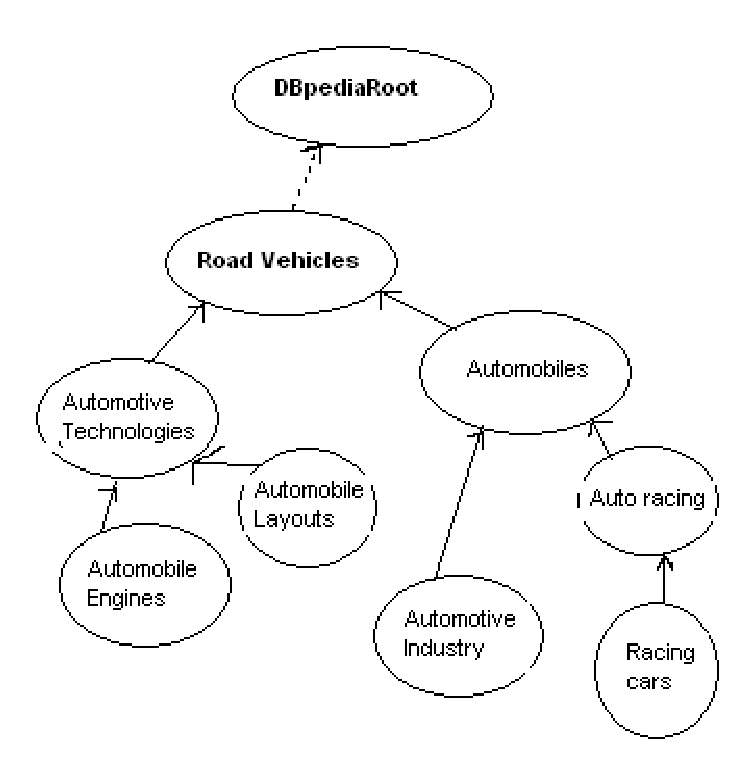
\includegraphics[width=90mm]{class_divergence.eps}
\caption{Abbrv. graphical representation of an automotive ontology}
\label{fig:class_divergence}
\end{figure}

Figure \ref{fig:class_divergence} illustrates the calculation of class
divergence. This sample abbreviated ontology that was created from the
DBpedia category heirarchy is rooted at the class
\textit{DBpediaRoot}. The arrows represent the inheritance
relationship between the classes in the topology.

Suppose we want to find the divergence $d_{class}$\textit{(Automotive
  Industry, Racing Cars)}. The \textit{Automotive Industry} is the
subclass of \textit{Automobiles} and \textit{Racing Cars} is the
subclass of \textit{Auto Racinng}. Therefore, the common ancestor for
these two can be determined as \textit{Automobiles} ($C$). They share
the path from \textit{Automobiles} to the $root$. So, the unnormalized
divergence \textit{d(Automotive Industry, root)} is 32 (calcuted from
the path to root), \textit{d(Automotive Industry, Automobiles)} is one
(dashed arrow), and \textit{d(Racing Cars, Automobiles)} is two
(dashed arrow). Suppose, the ontology tree height is calculated as
294. Thus, \textit{d(Automotive Industry, Racing Cars)} is 35, which
corresponds to a normalized value of $35/294$.

%-------------------------------------------------------------------------------
\subsection{SSQ Ontology Matching}
\label{sec:oqom}

We use class divergence to calculate the relevance between a source
SSQ and a target SSQ associated with a QRM.  Each SSQ will have four
input classes, four output classes, and one realm.  We refer to the
sequence of these classes $\langle \Upsilon_1, ..., \Upsilon_4,
\Omega_1, ..., \Omega_4, R \rangle$ as the signature of an SSQ. If an
input or output class is unspecified in the query, it is associated
with the class $bottom$, which has no subclasses or individuals.

The relevance of QRM $Q$ with signature $\langle \Upsilon_{Q_1}, ...,
\Upsilon_{Q_4}, \\\Omega_{Q_1}, ... , \Omega_{Q_4}, R_Q\rangle$ to SSQ
$S$ with signature $\langle \Upsilon_{S_1}, ..., \Upsilon_{S_4},
\\\Omega_{S_1}, ... , \Omega_{S_4}, R_S \rangle$ is

\begin{eqnarray}
\label{qrmsimilarity}
 R(S,Q) = 1 - (d_{R} + d_{\Upsilon} + d_{\Omega})
\end{eqnarray}
\noindent where 
\begin{eqnarray}
d_{R} = \pi_9 d_{class}(R_S,R_Q) \nonumber
\end{eqnarray}
\begin{eqnarray}
d_{\Upsilon}  = \sum_{k=1}^4 {\pi_k} {d_{class}(\Upsilon_{S_k},\Upsilon_{Q_k})} \nonumber
\end{eqnarray}
\begin{eqnarray}
 d_{\Omega} = \sum_{j=1}^4 \pi_{4+j} d_{class}(\Omega_{S_j},\Omega_{Q_j})  \nonumber
\end{eqnarray}
\noindent the weights ${\pi}_k$ of the property hasRealm and other context properties satisfies the conditions 
\begin{equation}
\label{piconstraint1}
\sum_{k=1}^{9} {{\pi}_k} = 1
\end{equation}
\noindent and for $1 \leq i \leq 9$

\begin{equation}
\label{piconstraint2}
{\pi}_i > 0
\end{equation}

If an SSQ and a QRM have identical classes for all inputs and their
realms then the QRM relevance value will be one. Otherwise, the
relevance of the QRM will be in the range $[0, 1)$. 

%-------------------------------------------------------------------------------
